\documentclass[12pt]{article}
\usepackage{geometry}
\usepackage{array}
\usepackage{graphicx}
\usepackage{multirow}
\usepackage{booktabs}
\usepackage{times}
\usepackage{float}
\usepackage{tikz}
\usetikzlibrary{matrix,calc, positioning, shapes, arrows}


%isolated term
%#1 - Optional. Space between node and grouping line. Default=0
%#2 - node
%#3 - filling color
\newcommand{\implicantsol}[3][0]{
    \draw[rounded corners=3pt, fill=#3, opacity=0.3] ($(#2.north west)+(135:#1)$) rectangle ($(#2.south east)+(-45:#1)$);
    }


%internal group
%#1 - Optional. Space between node and grouping line. Default=0
%#2 - top left node
%#3 - bottom right node
%#4 - filling color
\newcommand{\implicant}[4][0]{
    \draw[rounded corners=3pt, fill=#4, opacity=0.3] ($(#2.north west)+(135:#1)$) rectangle ($(#3.south east)+(-45:#1)$);
    }

%group lateral borders
%#1 - Optional. Space between node and grouping line. Default=0
%#2 - top left node
%#3 - bottom right node
%#4 - filling color
\newcommand{\implicantcostats}[4][0]{
    \draw[rounded corners=3pt, fill=#4, opacity=0.3] ($(rf.east |- #2.north)+(90:#1)$)-| ($(#2.east)+(0:#1)$) |- ($(rf.east |- #3.south)+(-90:#1)$);
    \draw[rounded corners=3pt, fill=#4, opacity=0.3] ($(cf.west |- #2.north)+(90:#1)$) -| ($(#3.west)+(180:#1)$) |- ($(cf.west |- #3.south)+(-90:#1)$);
}

%group top-bottom borders
%#1 - Optional. Space between node and grouping line. Default=0
%#2 - top left node
%#3 - bottom right node
%#4 - filling color
\newcommand{\implicantdaltbaix}[4][0]{
    \draw[rounded corners=3pt, fill=#4, opacity=0.3] ($(cf.south -| #2.west)+(180:#1)$) |- ($(#2.south)+(-90:#1)$) -| ($(cf.south -| #3.east)+(0:#1)$);
    \draw[rounded corners=3pt, fill=#4, opacity=0.3] ($(rf.north -| #2.west)+(180:#1)$) |- ($(#3.north)+(90:#1)$) -| ($(rf.north -| #3.east)+(0:#1)$);
}

%group corners
%#1 - Optional. Space between node and grouping line. Default=0
%#2 - filling color
\newcommand{\implicantcantons}[2][0]{
    \draw[rounded corners=3pt, opacity=.3] ($(rf.east |- 0.south)+(-90:#1)$) -| ($(0.east |- cf.south)+(0:#1)$);
    \draw[rounded corners=3pt, opacity=.3] ($(rf.east |- 8.north)+(90:#1)$) -| ($(8.east |- rf.north)+(0:#1)$);
    \draw[rounded corners=3pt, opacity=.3] ($(cf.west |- 2.south)+(-90:#1)$) -| ($(2.west |- cf.south)+(180:#1)$);
    \draw[rounded corners=3pt, opacity=.3] ($(cf.west |- 10.north)+(90:#1)$) -| ($(10.west |- rf.north)+(180:#1)$);
    \fill[rounded corners=3pt, fill=#2, opacity=.3] ($(rf.east |- 0.south)+(-90:#1)$) -|  ($(0.east |- cf.south)+(0:#1)$) [sharp corners] ($(rf.east |- 0.south)+(-90:#1)$) |-  ($(0.east |- cf.south)+(0:#1)$) ;
    \fill[rounded corners=3pt, fill=#2, opacity=.3] ($(rf.east |- 8.north)+(90:#1)$) -| ($(8.east |- rf.north)+(0:#1)$) [sharp corners] ($(rf.east |- 8.north)+(90:#1)$) |- ($(8.east |- rf.north)+(0:#1)$) ;
    \fill[rounded corners=3pt, fill=#2, opacity=.3] ($(cf.west |- 2.south)+(-90:#1)$) -| ($(2.west |- cf.south)+(180:#1)$) [sharp corners]($(cf.west |- 2.south)+(-90:#1)$) |- ($(2.west |- cf.south)+(180:#1)$) ;
    \fill[rounded corners=3pt, fill=#2, opacity=.3] ($(cf.west |- 10.north)+(90:#1)$) -| ($(10.west |- rf.north)+(180:#1)$) [sharp corners] ($(cf.west |- 10.north)+(90:#1)$) |- ($(10.west |- rf.north)+(180:#1)$) ;
}

%Empty Karnaugh map 4x4
\newenvironment{Karnaugh}%
{
\begin{tikzpicture}[baseline=(current bounding box.north),scale=0.8]
\draw (0,0) grid (4,4);
\draw (0,4) -- node [pos=0.7,above right,anchor=south west] {cd} node [pos=0.7,below left,anchor=north east] {ab} ++(135:1);
%
\matrix (mapa) [matrix of nodes,
        column sep={0.8cm,between origins},
        row sep={0.8cm,between origins},
        every node/.style={minimum size=0.3mm},
        anchor=8.center,
        ampersand replacement=\&] at (0.5,0.5)
{
                       \& |(c00)| 00         \& |(c01)| 01         \& |(c11)| 11         \& |(c10)| 10         \& |(cf)| \phantom{00} \\
|(r00)| 00             \& |(0)|  \phantom{0} \& |(1)|  \phantom{0} \& |(3)|  \phantom{0} \& |(2)|  \phantom{0} \&                     \\
|(r01)| 01             \& |(4)|  \phantom{0} \& |(5)|  \phantom{0} \& |(7)|  \phantom{0} \& |(6)|  \phantom{0} \&                     \\
|(r11)| 11             \& |(12)| \phantom{0} \& |(13)| \phantom{0} \& |(15)| \phantom{0} \& |(14)| \phantom{0} \&                     \\
|(r10)| 10             \& |(8)|  \phantom{0} \& |(9)|  \phantom{0} \& |(11)| \phantom{0} \& |(10)| \phantom{0} \&                     \\
|(rf) | \phantom{00}   \&                    \&                    \&                    \&                    \&                     \\
};
}%
{
\end{tikzpicture}
}

%Empty Karnaugh map 2x4
\newenvironment{Karnaughvuit}%
{
\begin{tikzpicture}[baseline=(current bounding box.north),scale=0.8]
\draw (0,0) grid (4,2);
\draw (0,2) -- node [pos=0.7,above right,anchor=south west] {$yz$} node [pos=0.7,below left,anchor=north east] {$x$} ++(135:1);
%
\matrix (mapa) [matrix of nodes,
        column sep={0.8cm,between origins},
        row sep={0.8cm,between origins},
        every node/.style={minimum size=0.3mm},
        anchor=4.center,
        ampersand replacement=\&] at (0.5,0.5)
{
                      \& |(c00)| 00         \& |(c01)| 01         \& |(c11)| 11         \& |(c10)| 10         \& |(cf)| \phantom{00} \\
|(r00)| 0             \& |(0)|  \phantom{0} \& |(1)|  \phantom{0} \& |(3)|  \phantom{0} \& |(2)|  \phantom{0} \&                     \\
|(r01)| 1             \& |(4)|  \phantom{0} \& |(5)|  \phantom{0} \& |(7)|  \phantom{0} \& |(6)|  \phantom{0} \&                     \\
|(rf) | \phantom{00}  \&                    \&                    \&                    \&                    \&                     \\
};
}%
{
\end{tikzpicture}
}

%Empty Karnaugh map 2x2
\newenvironment{Karnaughquatre}%
{
\begin{tikzpicture}[baseline=(current bounding box.north),scale=0.8]
\draw (0,0) grid (2,2);
\draw (0,2) -- node [pos=0.7,above right,anchor=south west] {b} node [pos=0.7,below left,anchor=north east] {a} ++(135:1);
%
\matrix (mapa) [matrix of nodes,
        column sep={0.8cm,between origins},
        row sep={0.8cm,between origins},
        every node/.style={minimum size=0.3mm},
        anchor=2.center,
        ampersand replacement=\&] at (0.5,0.5)
{
          \& |(c00)| 0          \& |(c01)| 1  \\
|(r00)| 0 \& |(0)|  \phantom{0} \& |(1)|  \phantom{0} \\
|(r01)| 1 \& |(2)|  \phantom{0} \& |(3)|  \phantom{0} \\
};
}%
{
\end{tikzpicture}
}

%Defines 8 or 16 values (0,1,X)
\newcommand{\contingut}[1]{%
\foreach \x [count=\xi from 0]  in {#1}
     \path (\xi) node {\x};
}

%Places 1 in listed positions
\newcommand{\minterms}[1]{%
    \foreach \x in {#1}
        \path (\x) node {1};
}

%Places 0 in listed positions
\newcommand{\maxterms}[1]{%
    \foreach \x in {#1}
        \path (\x) node {0};
}

%Places X in listed positions
\newcommand{\indeterminats}[1]{%
    \foreach \x in {#1}
        \path (\x) node {X};
}

\geometry{margin=1in}

\begin{document}

\begin{center}
    \textbf{HACETTEPE UNIVERSITY}\\
    \textbf{DEPARTMENT OF ELECTRICAL and ELECTRONICS ENGINEERING}\\
%%%%%%%%%%%%%%%%%%%%%%%%%%%%%%%%%%%%%%%%%%%%%%%%%%%%%%%%%%%%%%%%%%%%%%%%%%%%%%
%%%                            INSERT DATE HERE                            %%%
%%%%%%%%%%%%%%%%%%%%%%%%%%%%%%%%%%%%%%%%%%%%%%%%%%%%%%%%%%%%%%%%%%%%%%%%%%%%%%
    \textbf{ELE225 Fundamentals of Digital Systems Midterm Exam (Part A), 10 November 2025}
\end{center}

% Identification table

\begin{center}
\begin{tabular}{|p{2.2cm}|p{4.5cm}|p{3cm}|c|c|c|c|c|}
\hline
\textbf{Last name} & & \multirow{2}{*}{\textbf{SIGN:}} 
    & \multicolumn{5}{c|}{\textbf{Points}} \\ \cline{1-2}\cline{4-8}
\textbf{First name} & & 
    & Q1 & Q2 & Q3 & Q4 & Total \\ \hline

\textbf{Student \#} & & 
    &  &  &  &  &  \\ \hline
\end{tabular}
\end{center}

\noindent
\textbf{Q1.} A BCD-to-seven-segment decoder is a combinational circuit that converts a decimal digit in BCD to an appropriate code for the selection of segments in an indicator used to display the decimal digit in a familiar form. The seven outputs of the decoder $(a, b,c, d, e, f, g)$ select the corresponding segments in the display, as shown below. Use a truth table and by the use of Karnaugh maps, find the minimal SOP form of the outputs. Use don't care conditions, if any. The word displayed is "bArCELOnA".

\vspace{-1em}

\begin{center}
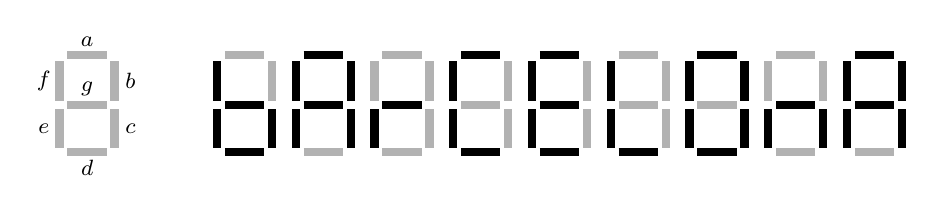
\begin{tikzpicture}
    \draw[black,opacity=.3,line width=3pt] (0,0) --+ (0,.5); %b
    \draw[black,opacity=.3,line width=3pt] (0,.6) --+ (0,.5); %a
    \draw[xshift=.7cm,black,opacity=.3,line width=3pt] (0,0) --+ (0,.5); %g
    \draw[xshift=.7cm,black,opacity=.3,line width=3pt] (0,.6) --+ (0,.5); %f
    \draw[black,opacity=.3,line width=3pt] (.1,1.18) --+ (.5,0); %c
    \draw[black,opacity=.3,line width=3pt] (.1,-.05) --+ (.5,0); %e
    \draw[black,opacity=.3,line width=3pt] (.1,.55) --+ (.5,0); %d
    \node at (-0.2, 0.85) {\footnotesize $f$};
    \node at (-0.2, 0.25) {\footnotesize $e$};
    \node at (0.35, 1.35) {\footnotesize $a$};
    \node at (0.35, 0.75) {\footnotesize $g$};
    \node at (0.35,-0.25) {\footnotesize $d$};
    \node at (0.9, 0.85) {\footnotesize $b$};
    \node at (0.9, 0.25) {\footnotesize $c$};

    \draw[black,line width=3pt] (2,0) --+ (0,.5); %b
    \draw[black,line width=3pt] (2,.6) --+ (0,.5); %a
    \draw[xshift=.7cm,black,line width=3pt] (2,0) --+ (0,.5); %g
    \draw[xshift=.7cm,black,opacity=.3,line width=3pt] (2,.6) --+ (0,.5); %f
    \draw[black,opacity=.3,line width=3pt] (2.1,1.18) --+ (.5,0); %c
    \draw[black,line width=3pt] (2.1,-.05) --+ (.5,0); %e
    \draw[black,line width=3pt] (2.1,.55) --+ (.5,0); %d

    \draw[black,line width=3pt] (3,0) --+ (0,.5); %b
    \draw[black,line width=3pt] (3,.6) --+ (0,.5); %a
    \draw[xshift=.7cm,black,line width=3pt] (3,0) --+ (0,.5); %g
    \draw[xshift=.7cm,black,line width=3pt] (3,.6) --+ (0,.5); %f
    \draw[black,line width=3pt] (3.1,1.18) --+ (.5,0); %c
    \draw[black,opacity=.3,line width=3pt] (3.1,-.05) --+ (.5,0); %e
    \draw[black,line width=3pt] (3.1,.55) --+ (.5,0); %d

    \draw[black,line width=3pt] (4,0) --+ (0,.5); %b
    \draw[black,opacity=.3,line width=3pt] (4,.6) --+ (0,.5); %a
    \draw[xshift=.7cm,black,opacity=.3,line width=3pt] (4,0) --+ (0,.5); %g
    \draw[xshift=.7cm,black,opacity=.3,line width=3pt] (4,.6) --+ (0,.5); %f
    \draw[black,opacity=.3,line width=3pt] (4.1,1.18) --+ (.5,0); %c
    \draw[black,opacity=.3,line width=3pt] (4.1,-.05) --+ (.5,0); %e
    \draw[black,line width=3pt] (4.1,.55) --+ (.5,0); %d

    \draw[black,line width=3pt] (5,0) --+ (0,.5); %b
    \draw[black,line width=3pt] (5,.6) --+ (0,.5); %a
    \draw[xshift=.7cm,black,opacity=.3,line width=3pt] (5,0) --+ (0,.5); %g
    \draw[xshift=.7cm,black,opacity=.3,line width=3pt] (5,.6) --+ (0,.5); %f
    \draw[black,line width=3pt] (5.1,1.18) --+ (.5,0); %c
    \draw[black,line width=3pt] (5.1,-.05) --+ (.5,0); %e
    \draw[black,opacity=.3,line width=3pt] (5.1,.55) --+ (.5,0); %d

    \draw[black,line width=3pt] (6,0) --+ (0,.5); %b
    \draw[black,line width=3pt] (6,.6) --+ (0,.5); %a
    \draw[xshift=.7cm,black,opacity=.3,line width=3pt] (6,0) --+ (0,.5); %g
    \draw[xshift=.7cm,black,opacity=.3,line width=3pt] (6,.6) --+ (0,.5); %f
    \draw[black,line width=3pt] (6.1,1.18) --+ (.5,0); %c
    \draw[black,line width=3pt] (6.1,-.05) --+ (.5,0); %e
    \draw[black,line width=3pt] (6.1,.55) --+ (.5,0); %d

    \draw[black,line width=3pt] (7,0) --+ (0,.5); %b
    \draw[black,line width=3pt] (7,.6) --+ (0,.5); %a
    \draw[xshift=.7cm,black,opacity=.3,line width=3pt] (7,0) --+ (0,.5); %g
    \draw[xshift=.7cm,black,opacity=.3,line width=3pt] (7,.6) --+ (0,.5); %f
    \draw[black,opacity=.3,line width=3pt] (7.1,1.18) --+ (.5,0); %c
    \draw[black,line width=3pt] (7.1,-.05) --+ (.5,0); %e
    \draw[black,opacity=.3,line width=3pt] (7.1,.55) --+ (.5,0); %d

    \draw[black,line width=3pt] (8,0) --+ (0,.5); %b
    \draw[black,line width=3pt] (8,.6) --+ (0,.5); %a
    \draw[xshift=.7cm,black,line width=3pt] (8,0) --+ (0,.5); %g
    \draw[xshift=.7cm,black,line width=3pt] (8,.6) --+ (0,.5); %f
    \draw[black,line width=3pt] (8.1,1.18) --+ (.5,0); %c
    \draw[black,line width=3pt] (8.1,-.05) --+ (.5,0); %e
    \draw[black,opacity=.3,line width=3pt] (8.1,.55) --+ (.5,0); %d

    \draw[black,line width=3pt] (9,0) --+ (0,.5); %b
    \draw[black,opacity=.3,line width=3pt] (9,.6) --+ (0,.5); %a
    \draw[xshift=.7cm,black,line width=3pt] (9,0) --+ (0,.5); %g
    \draw[xshift=.7cm,black,opacity=.3,line width=3pt] (9,.6) --+ (0,.5); %f
    \draw[black,opacity=.3,line width=3pt] (9.1,1.18) --+ (.5,0); %c
    \draw[black,opacity=.3,line width=3pt] (9.1,-.05) --+ (.5,0); %e
    \draw[black,line width=3pt] (9.1,.55) --+ (.5,0); %d

    \draw[black,line width=3pt] (10,0) --+ (0,.5); %b
    \draw[black,line width=3pt] (10,.6) --+ (0,.5); %a
    \draw[xshift=.7cm,black,line width=3pt] (10,0) --+ (0,.5); %g
    \draw[xshift=.7cm,black,line width=3pt] (10,.6) --+ (0,.5); %f
    \draw[black,line width=3pt] (10.1,1.18) --+ (.5,0); %c
    \draw[black,opacity=.3,line width=3pt] (10.1,-.05) --+ (.5,0); %e
    \draw[black,line width=3pt] (10.1,.55) --+ (.5,0); %d
\end{tikzpicture}
\end{center}

\begin{minipage}[t]{0.45\textwidth}
\centering
\begin{tabular}{ |c|c|c|c|c|c|c|c| } 
    \hline
    $xyz$ & $a$ & $b$ & $c$ &$d$ & $e$ & $f$ & $g$ \\\hline
    $000$ & & & & & & & \\\hline
    $001$ & & & & & & & \\\hline
    $010$ & & & & & & & \\\hline
    $011$ & & & & & & & \\\hline
    $100$ & & & & & & & \\\hline
    $101$ & & & & & & & \\\hline
    $110$ & & & & & & & \\\hline
    $111$ & & & & & & & \\\hline
\end{tabular}

\vspace{1em}

\begin{minipage}{0.7\textwidth}
\begin{Karnaughvuit}
\end{Karnaughvuit}
\end{minipage}\begin{minipage}{0.3\textwidth}
$a=$
\end{minipage}

\vspace{-1em}

\begin{minipage}{0.7\textwidth}
\begin{Karnaughvuit}
\end{Karnaughvuit}
\end{minipage}\begin{minipage}{0.3\textwidth}
$b=$
\end{minipage}

\vspace{-1em}

\begin{minipage}{0.7\textwidth}
\begin{Karnaughvuit}
\end{Karnaughvuit}
\end{minipage}\begin{minipage}{0.3\textwidth}
$c=$
\end{minipage}

\end{minipage}
\hfill
\begin{minipage}[t]{0.5\textwidth}
\begin{minipage}{0.7\textwidth}
\begin{Karnaughvuit}
\end{Karnaughvuit}
\end{minipage}\begin{minipage}{0.3\textwidth}
$d=$
\end{minipage}

\vspace{-1em}

\begin{minipage}{0.7\textwidth}
\begin{Karnaughvuit}
\end{Karnaughvuit}
\end{minipage}\begin{minipage}{0.3\textwidth}
$e=$
\end{minipage}

\vspace{-1em}

\begin{minipage}{0.7\textwidth}
\begin{Karnaughvuit}
\end{Karnaughvuit}
\end{minipage}\begin{minipage}{0.3\textwidth}
$f=$
\end{minipage}

\vspace{-1em}

\begin{minipage}{0.7\textwidth}
\begin{Karnaughvuit}
\end{Karnaughvuit}
\end{minipage}\begin{minipage}{0.3\textwidth}
$g=$
\end{minipage}

\end{minipage}

\newpage

\noindent \textbf{Q2.} \textbf{a.} The numbers below are  12-bit unsigned binary numbers. Perform the operations step by step and show your work. Determine whether an overflow occurs.

\begin{minipage}[t]{0.45\textwidth}
\large
\vspace{0.5em}
\begin{verbatim}
 101001001001
 101010001010
\end{verbatim}
\vspace{-1.75em}
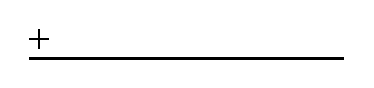
\begin{tikzpicture}
\draw[black,line width=1pt] (0,0.25) -- (0.25,0.25); %d
\draw[black,line width=1pt] (0.125,0.125) -- (0.125,0.375); %d
\draw[black,line width=1pt] (0,0) -- (4,0); %d
\end{tikzpicture}

\vspace{1em}

\noindent {\normalsize Did an overflow occur? YES / NO

\vspace{-0.5em}

Why?}
\end{minipage}
\hfill
\begin{minipage}[t]{0.45\textwidth}
\large
\vspace{0.5em}
\begin{verbatim}
 100111010101
 001010001010
\end{verbatim}
\vspace{-1.75em}
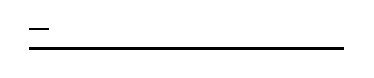
\begin{tikzpicture}
\draw[black,line width=1pt] (0,0.25) -- (0.25,0.25); %d
\draw[black,line width=1pt] (0,0) -- (4,0); %d
\end{tikzpicture}

\vspace{1em}

\noindent {\normalsize Did an overflow occur? YES / NO

\vspace{-0.5em}

Why?}
\end{minipage}

\vspace{4em}

\noindent \textbf{b.} The numbers below are 2's complement 12-bit binary numbers. Perform the operations step by step and show your work. Determine whether an overflow occurs.

\begin{minipage}[t]{0.45\textwidth}
\large
\vspace{0.5em}
\begin{verbatim}
 110100110101
 010001010001
\end{verbatim}
\vspace{-1.75em}
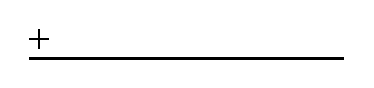
\begin{tikzpicture}
\draw[black,line width=1pt] (0,0.25) -- (0.25,0.25); %d
\draw[black,line width=1pt] (0.125,0.125) -- (0.125,0.375); %d
\draw[black,line width=1pt] (0,0) -- (4,0); %d
\end{tikzpicture}

\vspace{1em}

\noindent {\normalsize Did an overflow occur? YES / NO

\vspace{-0.5em}

Why?}
\end{minipage}
\hfill
\begin{minipage}[t]{0.45\textwidth}
\large
\vspace{0.5em}
\begin{verbatim}
 111010011100
 000111010001
\end{verbatim}
\vspace{-1.75em}
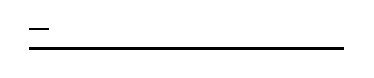
\begin{tikzpicture}
\draw[black,line width=1pt] (0,0.25) -- (0.25,0.25); %d
\draw[black,line width=1pt] (0,0) -- (4,0); %d
\end{tikzpicture}

\vspace{1em}

\noindent {\normalsize Did an overflow occur? YES / NO

\vspace{-0.5em}

Why?}
\end{minipage}

\vspace{4em}

\noindent \textbf{c.} You are to use a base-13 number system, where the digits are alphabetically ordered letters starting from A. Perform the following operation and show your work clearly.

\begin{minipage}[t]{0.45\textwidth}
\large
\vspace{0.5em}
\begin{verbatim}
 MAKE
 CAKE
\end{verbatim}
\vspace{-1.75em}
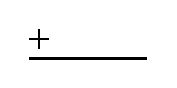
\begin{tikzpicture}
\draw[black,line width=1pt] (0,0.25) -- (0.25,0.25); %d
\draw[black,line width=1pt] (0.125,0.125) -- (0.125,0.375); %d
\draw[black,line width=1pt] (0,0) -- (1.5,0); %d
\end{tikzpicture}
\end{minipage}

\vspace{4em}

\noindent \textbf{d.} Find the result $(2306)_7-(43450)_7=(?)_7$ by taking the 7's complement. Show your work clearly.

%%%%%%%%%%%%%%%%%%%%%%%%%%%%%%%%%%%%%%%%%%%%%%%%%%%%%%%%%%%%%%%%%%%%%%%%%%%%%%
%%%                INSERT YOUR QUESTION HERE                               %%%
%%%%%%%%%%%%%%%%%%%%%%%%%%%%%%%%%%%%%%%%%%%%%%%%%%%%%%%%%%%%%%%%%%%%%%%%%%%%%%

\begin{figure}[H]
    \centering
%    \includegraphics[width=1\linewidth]{Ekran görüntüsü 2025-06-26 152205.png}
\end{figure}

\newpage

\noindent \textbf{Q3.} Using the minimum number of OR, AND, INVERT gates, reduce the following circuit to an equivalent form. Complement forms are not available.

\begin{figure}[H]
    \centering
    \includegraphics[width=1\linewidth]{chrome_HnhSOkvCDN.png}
\end{figure}

\vspace{15em}

\noindent \textbf{Q4.} We have a 3-variable Karnaugh map, and it is known that

\begin{itemize}
    \item There are \textbf{at least} two essential prime implicants: $ac$ and $bc$,
    \item The minimized SOP form has \textbf{exactly} three products of variables.
\end{itemize}

\noindent Write all possible combinations that satisfy these conditions in sum of minterms form (i.e., $\sum m_i$).

\newpage

\begin{center}
    \textbf{HACETTEPE UNIVERSITY}\\
    \textbf{DEPARTMENT OF ELECTRICAL and ELECTRONICS ENGINEERING}\\
    \textbf{ELE225 Fundamentals of Digital Systems Midterm Exam (Part B), 10 November 2025}
\end{center}

\begin{center}
\begin{tabular}{|p{2.2cm}|p{4.5cm}|p{3cm}|c|c|c|c|c|}
\hline
\textbf{Last name} & & \multirow{2}{*}{\textbf{SIGN:}} 
    & \multicolumn{5}{c|}{\textbf{Points}} \\ \cline{1-2}\cline{4-8}
\textbf{First name} & & 
    & Q1 & Q2 & Q3 & Q4 & Total \\ \hline

\textbf{Student \#} & & 
    &  &  &  &  &  \\ \hline
\end{tabular}
\end{center}

\noindent
\textbf{Q1.} The outputs of a 8x1 multiplexer is given [\textit{MISSING}].

\hfill

\noindent \textbf{a.} Design this multiplexer.

\vspace{15em}

\noindent \textbf{b.} Using the don't care conditions in the Karnaugh map, write the minimal SOP form.

\vspace{5em}

\noindent \textbf{c.} Design the circuit with a two-level NOR-only implementation using the don't care conditions you used in part b.

\newpage

\noindent \textbf{Q2.} Using the 4-bit adder below, implement a circuit that outputs 1 when \textbf{any} of the following conditions holds. (S$_3$: MSB, S$_0$: LSB)

\begin{itemize}
    \item S$_3>$ S$_1$,
    \item S$_3=$ S$_2 =$ S$_1=0$,
    \item if the decimal form of the sum is greater than 3 and less than 9.
\end{itemize}

\hfill

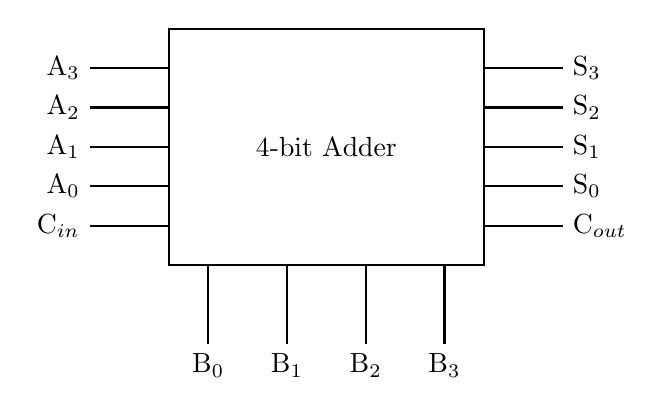
\begin{tikzpicture}[>=latex, thick]

% 4-bit adder block (rectangle)
\draw (0,0) rectangle (4,3);
\node at (2,1.5) {4-bit Adder};

% --- A inputs on the left side ---
\draw (-1,2.5) node[left]{A$_3$} -- (0,2.5);
\draw (-1,2.0) node[left]{A$_2$} -- (0,2.0);
\draw (-1,1.5) node[left]{A$_1$} -- (0,1.5);
\draw (-1,1.0) node[left]{A$_0$} -- (0,1.0);

% --- Carry in on the left side ---
\draw (-1,0.5) node[left]{C$_{in}$} -- (0,0.5);

% --- B inputs on the bottom side ---
\draw (0.5,-1) node[below]{B$_0$} -- (0.5,0);
\draw (1.5,-1) node[below]{B$_1$} -- (1.5,0);
\draw (2.5,-1) node[below]{B$_2$} -- (2.5,0);
\draw (3.5,-1) node[below]{B$_3$} -- (3.5,0);

% --- Sum outputs on the right side ---
\draw (4,2.5) -- (5,2.5) node[right]{S$_3$};
\draw (4,2.0) -- (5,2.0) node[right]{S$_2$};
\draw (4,1.5) -- (5,1.5) node[right]{S$_1$};
\draw (4,1.0) -- (5,1.0) node[right]{S$_0$};

% --- Carry out on the right side ---
\draw (4,0.5) -- (5,0.5) node[right]{C$_{out}$};

\end{tikzpicture}

\hfill

\noindent Minimal SOP form: $F=$

\newpage

\noindent \textbf{Q3.} Find the minimal SOP expression manually [\textit{MISSING}].

\vspace{20em}

\noindent \textbf{Q4.} [\textit{MISSING}].

\end{document}